\documentclass[10pt,twocolumn]{article}
\usepackage[margin=0.72in]{geometry}
\usepackage{booktabs}
\usepackage{amsmath}
\usepackage{amssymb}
\usepackage{newtxtext,newtxmath}
\usepackage{microtype}
\usepackage[font=small,labelfont=bf,skip=5pt]{caption}
\usepackage{titlesec}
\usepackage{fancyhdr}
\usepackage{algorithm}
\usepackage{algpseudocode}
\renewcommand{\algorithmicrequire}{\textbf{Input:}}
\renewcommand{\algorithmicensure}{\textbf{Output:}}
\usepackage{graphicx}
\usepackage{tikz}
\usepackage{pgfplots}
\usepgfplotslibrary{fillbetween}
\pgfplotsset{compat=1.18,
  every axis/.append style={
    ymajorgrids, grid style={gray!22,line width=0.3pt},
    axis line style={gray!70}, tick style={gray!70}}}
\usepackage{flushend}
\usepackage[hidelinks]{hyperref}
\usepackage{xcolor}
\definecolor{oldc}{RGB}{158,31,54}
\definecolor{newc}{RGB}{21,96,130}
\definecolor{new2c}{RGB}{94,155,183}
\renewcommand{\topfraction}{0.96}
\renewcommand{\dbltopfraction}{0.96}
\renewcommand{\textfraction}{0.03}
\renewcommand{\floatpagefraction}{0.9}
\renewcommand{\dblfloatpagefraction}{0.9}
\setlength{\textfloatsep}{6pt plus 1pt minus 2pt}
\setlength{\dbltextfloatsep}{6pt plus 1pt minus 2pt}

\titleformat{\section}{\large\bfseries\color{newc}}{\thesection}{0.6em}{}
\titlespacing*{\section}{0pt}{9pt plus 2pt}{4pt}
\titleformat{\subsection}{\normalsize\bfseries\color{newc!85!black}}{\thesubsection}{0.6em}{}
\titlespacing*{\subsection}{0pt}{7pt plus 2pt}{3pt}

\pagestyle{fancy}
\fancyhf{}
\fancyhead[L]{\footnotesize\itshape Dwell-Adaptive RF Signal Classification from Duration-Complete Synthetic Data}
\fancyhead[R]{\footnotesize\thepage}
\renewcommand{\headrulewidth}{0.3pt}
\fancypagestyle{plain}{\fancyhf{}\fancyfoot[C]{\footnotesize\thepage}\renewcommand{\headrulewidth}{0pt}}

\hypersetup{pdftitle={Dwell-Adaptive RF Signal Classification from Duration-Complete Synthetic Data},pdfauthor={John Elliott}}

\newcommand{\method}{DACS}

\title{\vspace{-4mm}\textbf{Dwell-Adaptive RF Signal Classification from\\Duration-Complete Synthetic Data}}
\author{\textbf{John Elliott}\\[1pt]\small Independent Researcher\\[0pt]\footnotesize\texttt{JohnElliott@journalcorrespondence.com}\\[4pt]\rule{0.72\textwidth}{0.4pt}}
\date{\vspace{-3mm}\small July 31, 2026}

\begin{document}
\maketitle

\begin{abstract}
The transmitters that matter most---drone control links, intermittent
interferers, frequency hoppers---announce themselves for less than a
millisecond at a time, while a spectrum monitor can watch only one slice of
the band at once: glance briefly and a hopper is indistinguishable from a
blip or from nothing; stare long enough to be sure and the rest of the band
goes unwatched. Deep I/Q classifiers inherit the worst half of this bargain
because they are trained on windows fixed in \emph{samples}, spanning
microseconds of millisecond-scale structure; the failure is one of evidence,
not modeling, and no architecture can learn rhythm its training windows never
contained. We present \method{} (Dwell-Adaptive Classification from
duration-complete Synthesis), an architecture with a sense of
time: one weight-shared, fully-convolutional-in-time network that reads a
capture at any dwell, with three heads giving it three faculties---a
prototype head that knows the class, a masked denoising autoencoder that
knows the channel (its target the true clean signal, silences included),
and a confidence head that knows itself---so that listening longer becomes
an action the classifier takes, capture by capture, rather than a
compromise fixed at design time. The capability is learnable only from
data in which time is a controlled variable: synthetic captures long
enough to hold each protocol's timing, silences retained as
class-conditional evidence, each paired with its clean reference.
With architecture, optimizer, and budget frozen, duration-complete training
alone lifts 7-class balanced accuracy from 0.503 to 0.954 at 1\,ms dwell and
1.000 at 10\,ms across two seeds, while architecture substitution, tripled
budget, and worst-case reweighting on fixed-window data all fail; a
companion analysis shows why standard worst-cell metrics could not even have
displayed the win. Training cost is linear in dwell.
\end{abstract}

{\small\noindent\textbf{Index terms---}RF signal classification, selective
classification, anytime inference, synthetic training data, frequency
hopping.\par}\vspace{4pt}

\section{Introduction}
The air around every airport fence, factory floor, and city block carries
transmitters no one can see---and the ones that matter most, the drone
control link, the interferer that kills a production line three packets at a
time, announce themselves for less than a millisecond before hopping
somewhere else. A spectrum monitor can listen to only one slice of that air
at a time, so it faces an impossible bargain: glance briefly and a frequency
hopper is indistinguishable from a harmless blip---or from nothing at
all---while staring long enough to be certain leaves the rest of the band
unwatched. Deep classifiers \cite{oshea2016,oshea2018} should resolve this
bargain, but trained on fixed-length windows that span microseconds of
millisecond-scale structure, they inherit its worst half: they answer
instantly, and they answer wrong, on exactly the signals they exist to
catch.

This failure looks like a modeling problem and has been attacked as
one---bigger networks, longer training, cleverer losses---but it is an
evidence problem: burst protocols are defined by rhythms measured in
milliseconds, GSM's 4.6\,ms frame \cite{ts45002}, Bluetooth's 625\,$\mu$s
slot cadence \cite{btcore}, while fixed-sample-count training windows span
microseconds of that rhythm, and no architecture, budget, or loss function
can recover structure its training windows physically never contained
(Fig.~\ref{fig:spectro}). Radio engineering's founding instinct is to
separate the signal from the noise---but burst protocols turn the instinct
against us: the silence between bursts is not noise to be rejected, it is
the signal's own rhythm, and every pipeline that discards ``empty'' windows
as invalid is, quite literally, separating the signal from itself---because
for spectro-temporal signals, the signal is sometimes the noise.

Since no fixed dwell can win---short looks miss identity, long looks miss
the band---the classifier itself must decide how long to listen. \method{}
(Dwell-Adaptive Classification from duration-complete Synthesis) is built
around that decision: one weight-shared network reads a capture at any
dwell, classifies it against prototypes, reconstructs what the clean signal
should have looked like (so silence is knowledge, not absence), and scores
its own reliability---escalating to a longer look only when that score
demands it. Training this sense of time requires data in which time is a
controlled variable: captures long enough to hold each protocol's timing,
with silence retained at its true class-conditional rate. Sec.~\ref{sec:motiv} verifies the
diagnosis quantitatively---including a third, less obvious casualty: the
worst-cell acceptance metrics of this domain are order statistics that
could not have displayed success even if a model achieved it.
Secs.~\ref{sec:model}--\ref{sec:synth} give the classifier and the data
technique; Sec.~\ref{sec:exp} then tests the diagnosis clause by clause:
swapping only the data moves balanced accuracy from 0.503 to 0.954 at
1\,ms dwell (1.000 at 10\,ms, two seeds), while every model-side
lever---architecture, budget, loss---fails to approach it.

\section{Related Work}
Deep I/Q classification varies architectures under a fixed observation
contract \cite{oshea2016,oshea2018}; \method{} changes the contract and
supplies the architecture built to exploit it. Its components are
established---prototype heads \cite{snell2017}, denoising and masked
autoencoders \cite{vincent2010,he2022}, trained confidence
\cite{devries2018,hendrycks2017}---but their composition realizes
selective prediction \cite{geifman2017} and early exiting
\cite{teerapittayanon2016,huang2018} along a new axis: physical
observation time rather than depth, with calibration \cite{guo2017}
governing escalation.

\begin{figure*}[t]
\centering
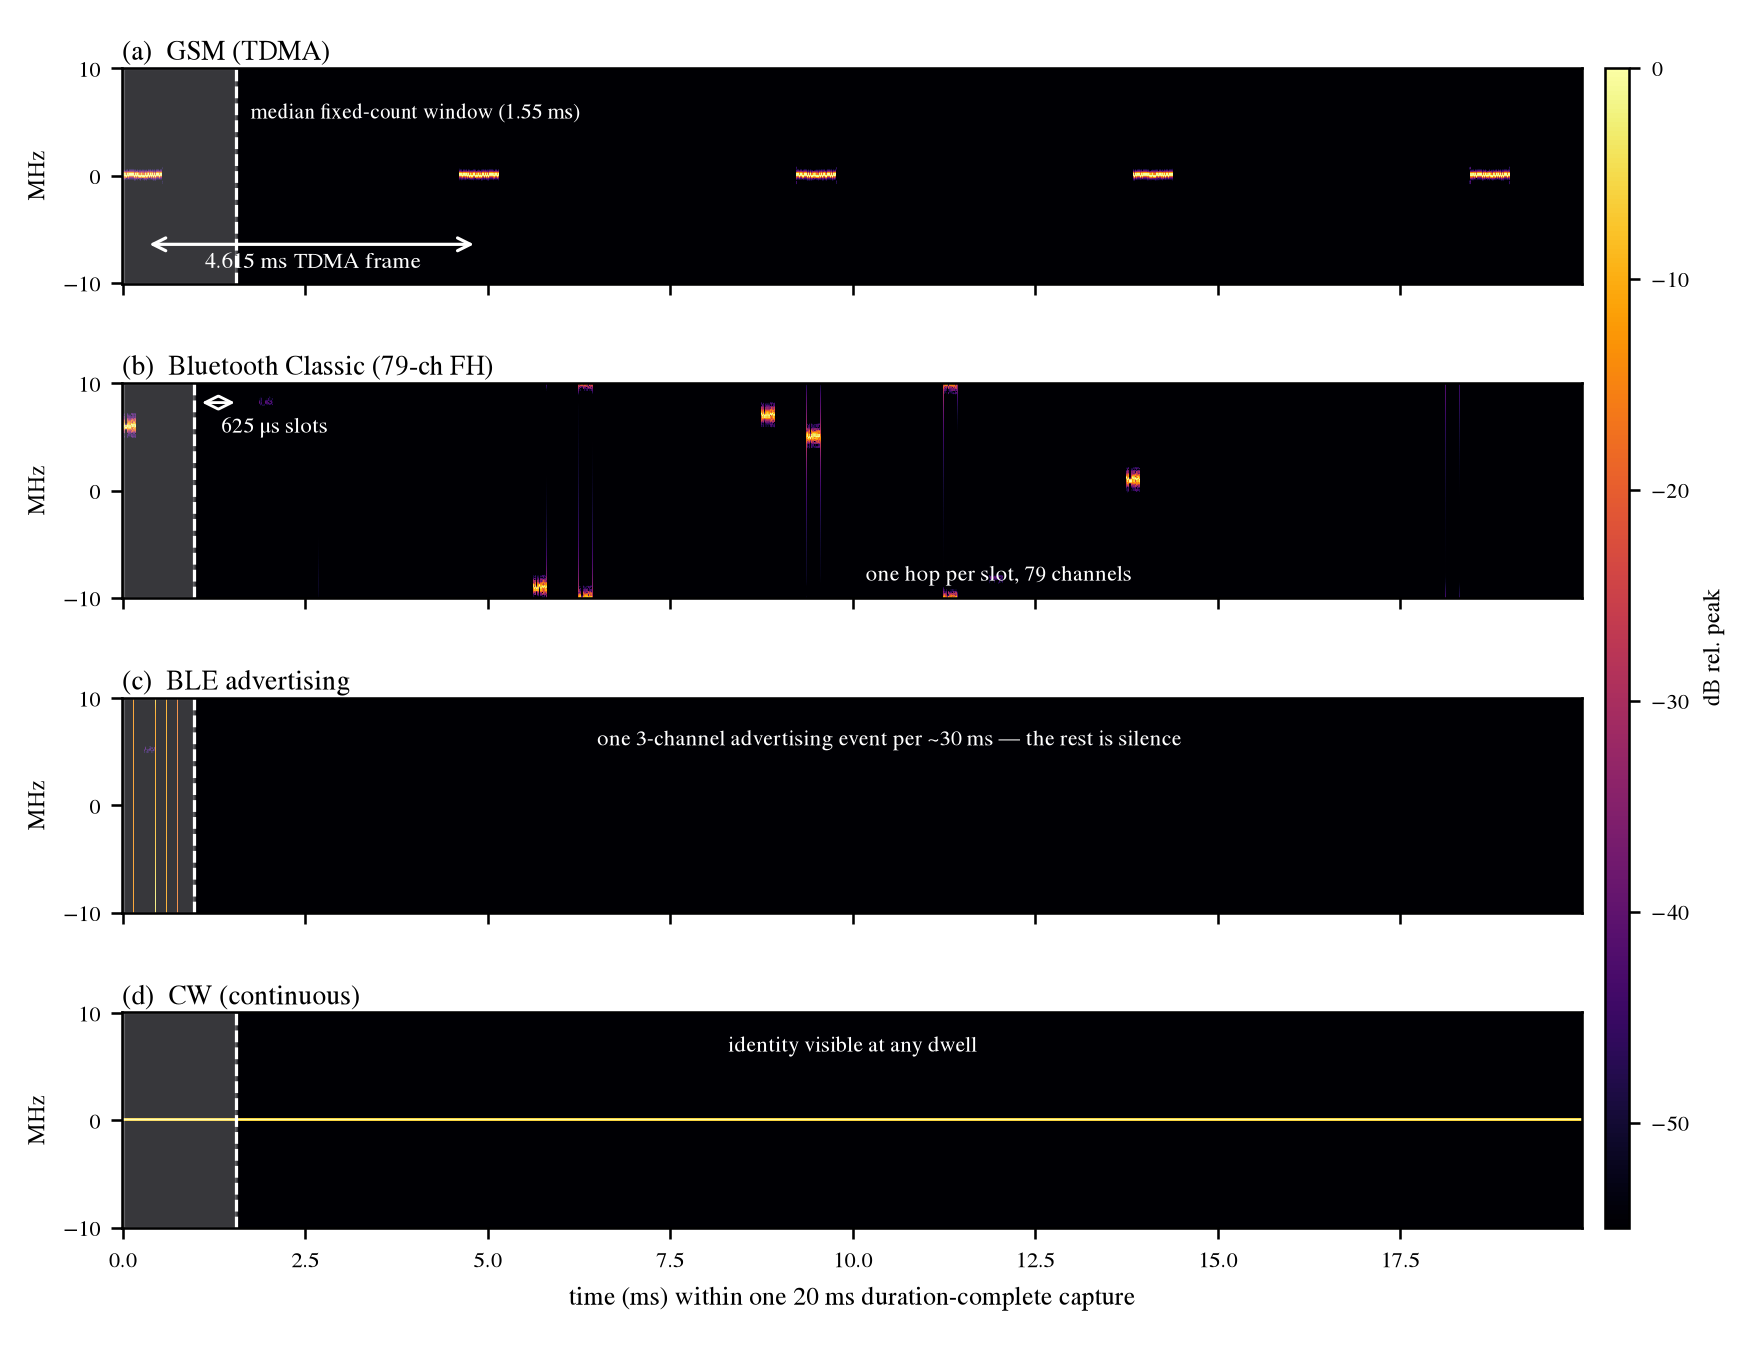
\includegraphics[width=0.64\textwidth]{fig_spectrograms.png}
\caption{\textbf{Class identity lives at timescales a fixed-sample-count
window rarely contains.} Spectrograms of single 20\,ms duration-complete
captures (clean synthesis, 20\,Msps): (a) GSM, (b) Bluetooth Classic,
(c) BLE advertising, (d) CW. Shading marks the median fixed-count window (16{,}384 samples,
1--200\,Msps sweep): within it, GSM shows at most one burst, Classic at
most one hop, BLE one event or pure silence. The 20\,ms capture contains
the discriminants: TDMA framing \cite{ts45002}, slot-clocked hopping and
sparse advertising \cite{btcore}, continuity for CW.}
\label{fig:spectro}
\end{figure*}

\section{Problem Analysis}
\label{sec:motiv}
Each claim of the diagnosis is checkable. We check them on the
\emph{fixed-count control corpus}: captures of 16{,}384 samples at rates
swept over 1--200\,Msps (median TDMA-class window 1.55\,ms), constructed to
instantiate the prevailing convention with the same classes and impairment
envelope as our method's corpus; we call such data \emph{duration-starved}.
Throughout, \emph{worst-window balanced accuracy} denotes the minimum over
the corpus's three window tiers (4{,}096/8{,}192/16{,}384 samples) of
7-class balanced accuracy.

\textbf{The windows really are empty.} Against the stationary expectation
that the first quarter of a capture holds $25\%$ of its energy, 37\% of GSM
captures hold ${<}10\%$ of capture energy in their first 4{,}096 samples
(Fig.~\ref{fig:diag}a aggregates all GSM configurations; burst-mode
configurations individually range 40--48\%, the always-on broadcast
carrier ${\approx}0\%$; block crest factor $39\times$); frequency-hopped
captures 23\%; DSSS 24\%; continuous classes ${\approx}0\%$. Conventional
pipelines reject these windows as invalid---discarding
$P(\text{silence}\mid\text{class})$, the statistic that a prior-optimal
analysis shows is alone worth balanced accuracy near 0.93.

\textbf{Energy is not the limit; rhythm is.} The continuously transmitting
GSM configuration (loaded broadcast carrier)---never empty---still yields
only 0.54 recall on the shortest window tier under the feature-engineered
baseline of Sec.~\ref{sec:exp} (mean over its 24 tuned configurations).
The GSM/Bluetooth discriminant is frame timing versus hop timing, both
invisible inside a sub-millisecond span, exactly as the diagnosis
predicts.

\textbf{Success could not even be displayed.} Acceptance criteria for
deployed classifiers often take the form of minimum recall over
(configuration$\times$condition) cells. With $J$ cells of $n$ evaluation
rows the displayed value is $\mathbb{E}[\min_j \hat p_j]$,
$\hat p_j \sim \mathrm{Bin}(n,p)/n$; for a representative design with
$J{=}124$ cells of $n{=}16$ (e.g., 31 configurations crossed with 4
conditions), true per-cell recall 0.95/0.97/0.99 reads as 0.77/0.82/0.89
(Fig.~\ref{fig:diag}b): a solved system reports 0.8. The remedy is
adequate cells, not a different statistic: at $J{=}34$, $n{=}96$, a true
0.97 displays as 0.93. We adopt per-configuration cells of $n{=}96$ per
dwell throughout, reporting balanced accuracy alongside the minimum
cell.

\begin{figure*}[t]
\centering
\begin{minipage}[t]{0.46\textwidth}
\vspace{0pt}\centering
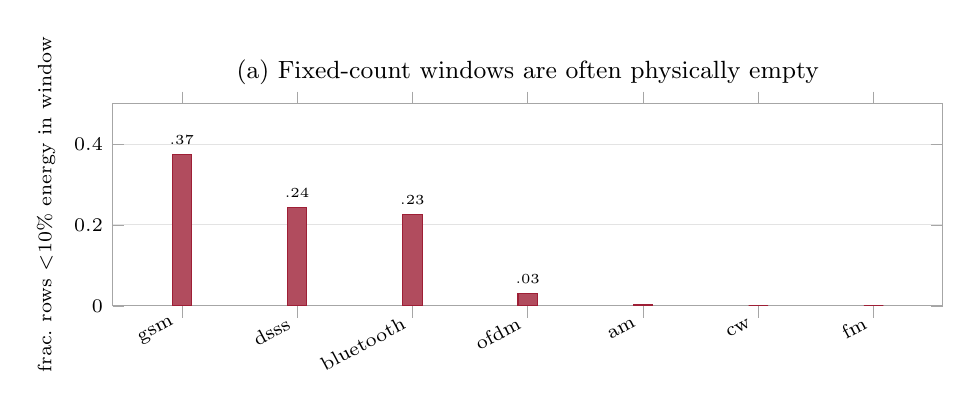
\begin{tikzpicture}
\begin{axis}[width=\linewidth,height=4.15cm,ybar,
  bar width=7pt, ymin=0, ymax=0.5,
  symbolic x coords={gsm,dsss,bluetooth,ofdm,am,cw,fm},
  xtick=data, x tick label style={font=\scriptsize,rotate=28,anchor=east},
  ylabel={\scriptsize frac.\ rows $<$10\% energy in window},
  ylabel style={font=\scriptsize}, tick label style={font=\scriptsize},
  title={\small (a) Fixed-count windows are often physically empty},
  title style={font=\small,yshift=-1mm}]
\addplot[fill=oldc!80,draw=oldc] coordinates
  {(gsm,0.374) (dsss,0.243) (bluetooth,0.226) (ofdm,0.031)
   (am,0.002) (cw,0.0) (fm,0.0)};
\node[font=\tiny,above] at (axis cs:gsm,0.374) {.37};
\node[font=\tiny,above] at (axis cs:dsss,0.243) {.24};
\node[font=\tiny,above] at (axis cs:bluetooth,0.226) {.23};
\node[font=\tiny,above] at (axis cs:ofdm,0.031) {.03};
\end{axis}
\end{tikzpicture}
\end{minipage}\hfill
\begin{minipage}[t]{0.50\textwidth}
\vspace{0pt}\centering
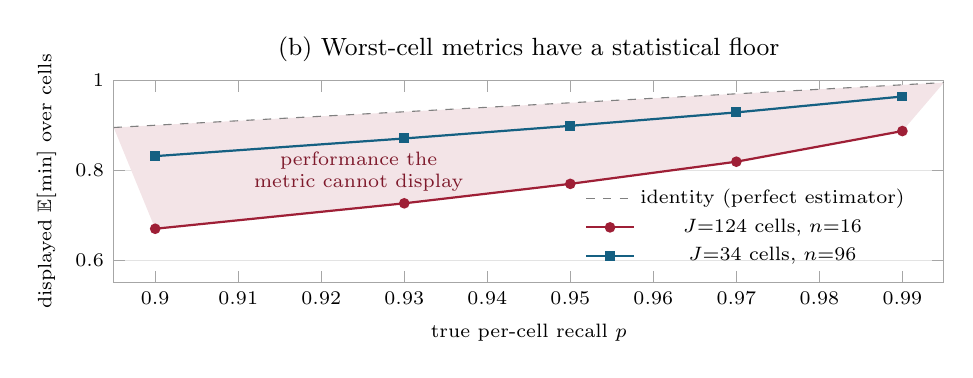
\begin{tikzpicture}
\begin{axis}[width=\linewidth,height=4.15cm,
  xmin=0.895,xmax=0.995,ymin=0.55,ymax=1.0,
  xlabel={\scriptsize true per-cell recall $p$},
  ylabel={\scriptsize displayed $\mathbb{E}[\min]$ over cells},
  xlabel style={font=\scriptsize}, ylabel style={font=\scriptsize},
  tick label style={font=\scriptsize},
  legend style={font=\scriptsize,at={(0.97,0.03)},anchor=south east,draw=none,
    fill=none},
  title={\small (b) Worst-cell metrics have a statistical floor},
  title style={font=\small,yshift=-1mm}]
\addplot[dashed,gray,name path=ident] coordinates
  {(0.895,0.895) (0.995,0.995)};
\addlegendentry{identity (perfect estimator)}
\addplot[thick,oldc,mark=*,mark size=1.5pt,name path=leg] coordinates
  {(0.90,0.6697) (0.93,0.7263) (0.95,0.7696) (0.97,0.8189) (0.99,0.8871)};
\addlegendentry{$J{=}124$ cells, $n{=}16$}
\addplot[oldc!12,forget plot] fill between[of=ident and leg];
\addplot[thick,newc,mark=square*,mark size=1.4pt] coordinates
  {(0.90,0.8313) (0.93,0.8706) (0.95,0.8987) (0.97,0.9286) (0.99,0.9640)};
\addlegendentry{$J{=}34$ cells, $n{=}96$}
\node[font=\scriptsize,oldc!80!black,align=center]
  at (axis cs:0.9245,0.796) {performance the\\metric cannot display};
\end{axis}
\end{tikzpicture}
\end{minipage}
\caption{\textbf{The premises, measured.} (a) Fraction of fixed-count
corpus rows whose scored window contains ${<}10\%$ of capture energy: the
hardest classes are frequently \emph{not in the window}. (b) Monte Carlo
readout ($2{\times}10^4$ draws) of minimum-over-cells metrics: small-$n$
cells cap what any model can \emph{display}, independent of its true
performance.}
\label{fig:diag}
\end{figure*}

\section{Method}
\label{sec:model}
The escape from the scanner's bargain is a network that treats dwell as a
decision variable---an instrument with three faculties: it knows the class,
it knows the channel, and it knows itself. A single spectro-temporal encoder (STFT front end; six
$3{\times}3$ convolution--GroupNorm--SiLU blocks, fully convolutional in
time, $32\times$ temporal downsampling; 1.0M parameters alone, 1.57M with
the decoder and heads below) feeds three heads (Fig.~\ref{fig:arch}). With
episode windows $x$ at dwells drawn from an ordered set
$\ell \in \{\ell_1 < \dots < \ell_K\}$ (we use $\{1, 2.5, 10\}$\,ms),
spectrogram $S_x$, random time-frame mask $m$, and class prototypes
computed from support embeddings \cite{snell2017}:
\begin{align*}
\mathcal{L} ={}& \mathcal{L}_{\mathrm{proto}}
 + \lambda_r \big\lVert D\!\big(E(m \odot S_x)\big) - S_{\mathrm{clean}}
   \big\rVert_1 \\
 &+ \lambda_d(t)\,\mathbb{E}_i\Big[\max_{\ell}
   \mathcal{L}_{\mathrm{proto}}\big(x_i^{(\ell)}\big)\Big]
 + \lambda_c\,\mathrm{BCE}\big(g(x), \mathbb{1}[\hat y = y]\big).
\end{align*}
$\mathcal{L}_{\mathrm{proto}}$ is episodic cross-entropy over squared
prototype distances with a learned temperature. The second term is a
masked denoising autoencoder \cite{vincent2010,he2022} with exact
supervision: $D\!\circ\!E$ must reproduce the capture's true clean
reference---not a proxy corruption of the input---so silence is a target
rather than an exclusion: for an idle stretch of a burst protocol the
correct reconstruction is the noise floor, and the network is graded on
knowing where the rhythm's rests fall
(Fig.~\ref{fig:dae} breaks this supervision down on a real capture).
Pseudocode for the episode loss is given in Algorithm~\ref{alg:train}. The third term trains the
shortest dwell against its hardest cases (max over dwells of the same
rows' episodic loss; prototypes detached; weight ramped linearly from
zero). The fourth trains $g$ to predict the classifier's own correctness
\cite{devries2018,hendrycks2017}. Optimization uses AdamW with cosine
annealing \cite{loshchilov2019}.

\textbf{Dwell policy.} At inference the system classifies at $\ell_1$ and
consults $g$: if calibrated confidence \cite{guo2017} clears a threshold
the answer is emitted; otherwise the capture extends to the next
dwell---selective classification \cite{geifman2017} in which the cost of
abstention is observation time, and the analogue of early exiting
\cite{teerapittayanon2016,huang2018} with physical time replacing depth.
Algorithm~\ref{alg:infer} states the policy; Fig.~\ref{fig:attr}
shows its payoff against observation time. The monitor spends milliseconds
only on the captures that demand them; everywhere else, the band stays
watched.

\begin{algorithm}[t]
\caption{\method{} training-episode loss. $N_C{=}7$ classes per
episode; $N_S$, $N_Q$ support/query captures per class; dwell set
$\{\ell_1{<}\dots{<}\ell_K\}$; $\lambda_r,\lambda_d(t),\lambda_c$
loss weights ($\lambda_d$ ramped). $\textsc{RandomSample}(S,N)$ draws
$N$ elements uniformly without replacement;
$\textsc{Window}(x,\ell)$ extracts a random-offset window of duration
$\ell$ from capture $x$; $\mathrm{Sp}$ is the STFT stack; $m$ a random
time-frame mask. $\mathcal{D}_k$ is the training subset with class $k$;
every capture $x$ is paired with its clean reference $\tilde{x}$.}
\label{alg:train}
\begin{algorithmic}\footnotesize
\Require training set $\mathcal{D}$ with clean pairs; encoder $E$,
decoder $D$, embedding $f_{\phi}$, confidence head $g$
\Ensure episode loss $J$
\State $\ell \gets \textsc{RandomSample}(\{\ell_1,\dots,\ell_K\},1)$
  \Comment{Draw episode dwell}
\For{$k$ in $\{1,\dots,N_C\}$}
  \State $S_k \gets \textsc{RandomSample}(\mathcal{D}_k, N_S)$;\;
    $Q_k \gets \textsc{RandomSample}(\mathcal{D}_k \setminus S_k, N_Q)$
    \Comment{Support/query captures}
  \State $x \gets \textsc{Window}(x,\ell)$ for every capture drawn
    \Comment{Empties retained}
  \State $\mathbf{c}_k \gets \tfrac{1}{N_S}\sum_{x \in S_k}
    f_{\phi}(\mathrm{Sp}(x))$ \Comment{Class prototype}
\EndFor
\State $J \gets \sum_{k}\sum_{x \in Q_k}
  \tfrac{1}{N_C N_Q}\,\mathrm{CE}\big({-}d(f_{\phi}(\mathrm{Sp}(x)),
  \mathbf{c}_{\cdot})\big)$ \Comment{Know the class}
\State $J \gets J + \lambda_r \lVert
  D(E(m \odot \mathrm{Sp}(x))) - \mathrm{Sp}(\tilde{x})
  \rVert_1$ \Comment{Know the channel: exact target}
\State $J \gets J + \lambda_d(t)\, \mathbb{E}_i\big[\max_{\ell'}
  \mathrm{CE}_i^{(\ell')}\big]$ \Comment{Worst dwell; amortized}
\State $J \gets J + \lambda_c\,\mathrm{BCE}\big(g(x),
  \mathbb{1}[\hat{y}=y]\big)$ \Comment{Know thyself}
\end{algorithmic}
\end{algorithm}

\begin{algorithm}[t]
\caption{Dwell-adaptive inference. $\tau$: confidence threshold
calibrated on held-out data; prototypes $\{\mathbf{c}_k\}$ from
enrollment; a capture keeps recording while the loop runs.}
\label{alg:infer}
\begin{algorithmic}\footnotesize
\Require capture stream $x$; dwell set
$\{\ell_1{<}\dots{<}\ell_K\}$; threshold $\tau$
\Ensure label $\hat{y}$, dwell spent
\For{$j$ in $\{1,\dots,K\}$}
  \State $z, g \gets f_{\phi}(\mathrm{Sp}(x[0{:}\ell_j])),\;
    g(x[0{:}\ell_j])$ \Comment{Re-encode the grown capture}
  \State $\hat{y} \gets \arg\min_k d(z, \mathbf{c}_k)$
    \Comment{Prototype decision}
  \If{$g \ge \tau$ \textbf{or} $j = K$}
    \State \Return $(\hat{y}, \ell_j)$ \Comment{Answer, or forced at max dwell}
  \EndIf
\EndFor \Comment{Otherwise: keep listening}
\end{algorithmic}
\end{algorithm}

\begin{figure*}[t]
\centering
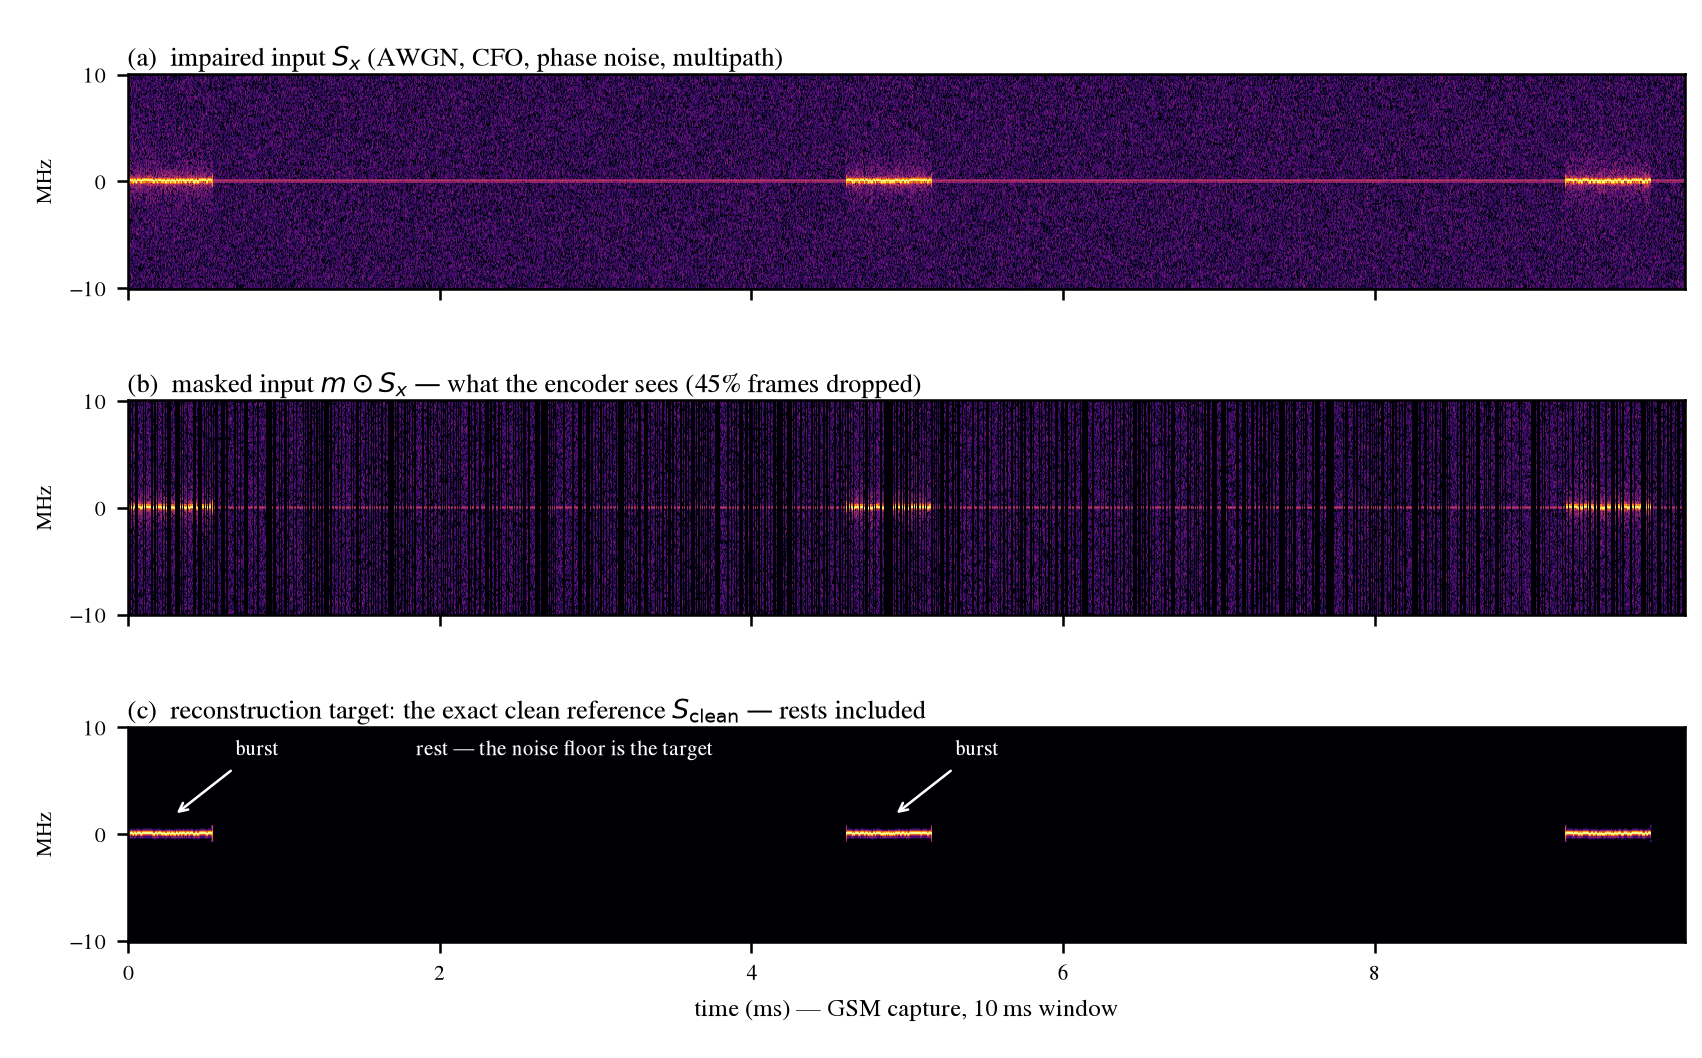
\includegraphics[width=0.64\textwidth]{fig_dae_breakdown.png}
\caption{\textbf{Exact-target denoising supervision, on a real GSM
capture.} (a) The impaired input: three TDMA bursts under AWGN, carrier
offset, phase noise, and multipath. (b) The masked view the encoder
receives. (c) The reconstruction target is the \emph{true clean
reference} from paired synthesis---not a corruption of the input---so
the rests between bursts are graded targets: the network must know where
the rhythm's silences fall. This supervision is unavailable to classic
denoising autoencoders and to any over-the-air dataset.}
\label{fig:dae}
\end{figure*}



\begin{figure*}[t]
\centering
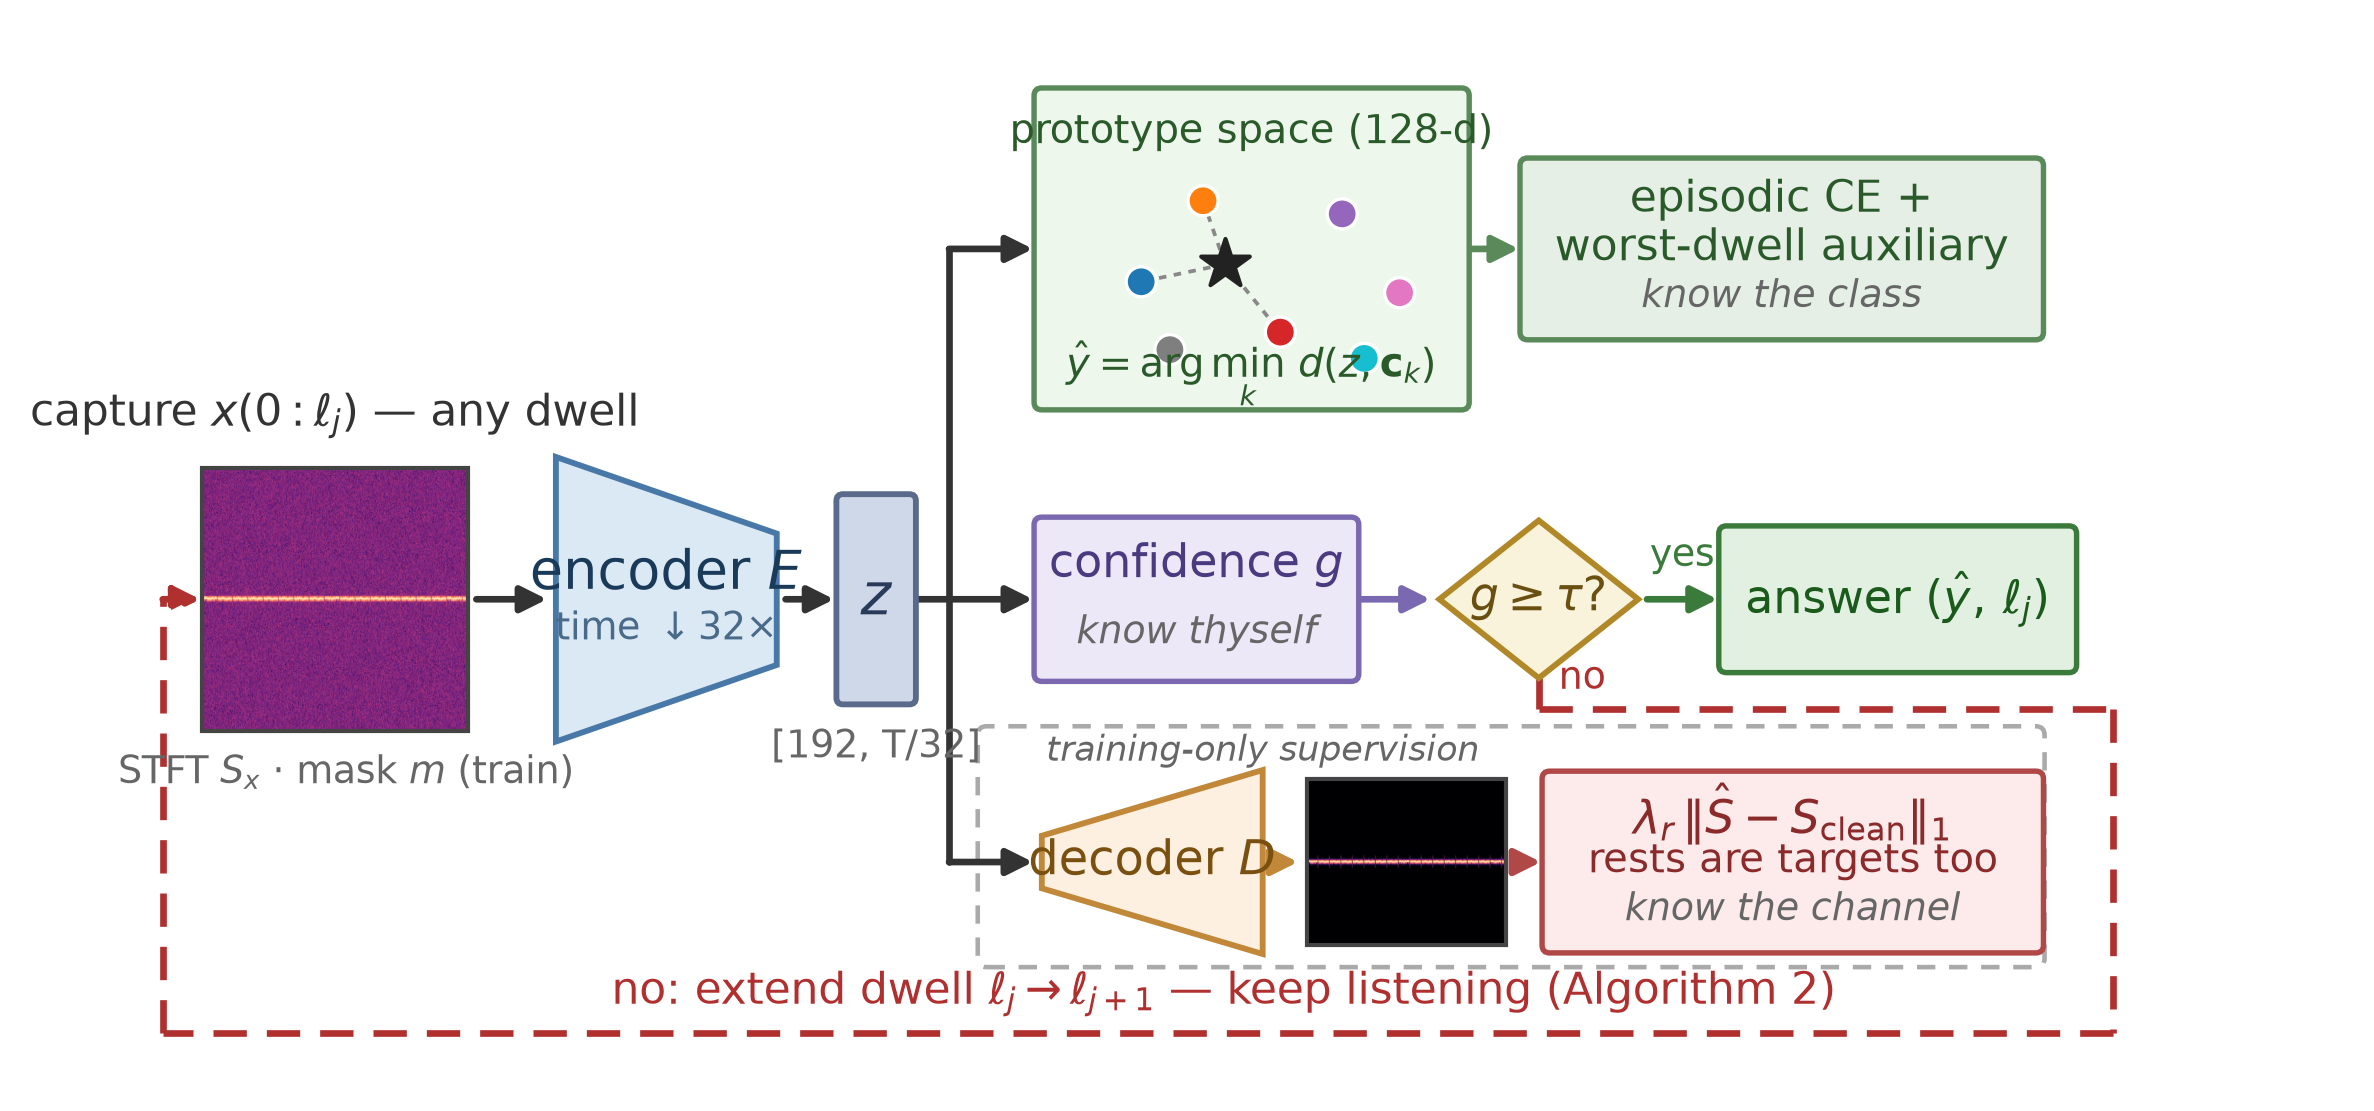
\includegraphics[width=0.86\textwidth]{fig_architecture.png}
\caption{\textbf{The \method{} network.} One shared spectro-temporal
encoder; three heads. The prototype embedding \cite{snell2017} carries
classification and preserves enrollment-based open-set operation; the
confidence head \cite{devries2018,geifman2017} drives the
answer-early/escalate dwell policy; the light decoder reconstructs the
clean reference's spectrogram under time-frame masking
\cite{he2022,vincent2010}, making silence a learning target and
regularizing against the shortcut overfit that duration-starved training
exhibits (Sec.~\ref{sec:exp}). The worst-case-over-dwell auxiliary trains
the shortest dwell against its hardest cases.}
\label{fig:arch}
\end{figure*}

\section{Dataset Generation}
\label{sec:synth}
Training requires corpora whose captures contain the structure of
Fig.~\ref{fig:spectro}; we summarize the technique and refer details to
the artifact. Every generator is \emph{index-pure}---a deterministic
function $y[n]=G(n)$ of absolute sample index---so arbitrary-duration
captures assemble byte-exactly from bounded, validated packet content.
Burst processes replay standards-derived packets \cite{btcore} on
unbounded timelines (slot-clocked keyed-hash hopping for Bluetooth
Classic; an event grid with the specification's \textit{advDelay} for
BLE), reproducing occupancy and timing \emph{statistics}; the
hop-selection kernel and payload variation are out of scope. Clean
captures are synthesized at native rates, resampled to 20\,Msps, and
impaired by a seeded receiver chain (AWGN at $U(-5,45)$\,dB SNR on
active-sample power, carrier offset, phase noise, IQ imbalance, DC,
multipath), yielding the row-aligned clean/impaired pairs of
Fig.~\ref{fig:dae}. Training windows are drawn by duration at random
offsets; empty windows are retained.

\section{Experiments and Results}
\label{sec:exp}
The diagnosis of Sec.~1 makes falsifiable predictions: swapping the data
should solve the problem; improving the model should not. We test both.

\textbf{Setup.} Seven classes (\texttt{am, bluetooth, cw, dsss, fm, gsm,
ofdm}) spanning 34 waveform configurations; 8{,}704 captures of 20\,ms,
96 evaluation rows per configuration (160 further captures per
configuration for training); impairments as in Sec.~\ref{sec:synth}. The
fixed-count control corpus is that of Sec.~\ref{sec:motiv}. Training
budget denotes the number of episodic updates (7-way, 5-shot/5-query;
dwell drawn uniformly per episode); the base budget is 8{,}000 episodes
and ``$3\times$'' is 24{,}000. Optimization: AdamW \cite{loshchilov2019},
cosine annealing, peak learning rate $2{\times}10^{-3}$; loss weights
$\lambda_r{=}0.3$, $\lambda_d{=}0.15$ (linear ramp over the first tenth of
training), $\lambda_c{=}0.1$. Evaluation classifies the capture-initial
window of each evaluation row at each dwell, with class prototypes
computed from 64 training captures per class under the identical protocol
on both corpora.

\textbf{Prediction 1: the data solves it.} Holding the encoder (1.0M
parameters, prototype loss only---no reconstruction, worst-case, or
confidence terms), optimizer, and budget fixed and swapping only the
corpus (Fig.~\ref{fig:attr}): balanced accuracy rises from 0.503 on the
shortest fixed-count tier to 0.954 at 1\,ms dwell, and from 0.682 to
1.000 at the longest tier vs.\ 10\,ms, with every class including GSM and
Bluetooth at recall 1.000 at 10\,ms; an independent seed reproduces
0.958/0.972/1.000. Criteria fixed before the runs executed
(GSM and BT ${\ge}0.85$ at 10\,ms; short-dwell balanced ${\ge}$ the
control level; monotone recall in dwell) all passed on both seeds.
Because the control corpus sweeps sample rate, its tiers are matched to
dwells by rank (shortest/mid/longest), not by physical duration, which
fixed-count data cannot hold constant.

\textbf{Prediction 2: the model does not} (Table~\ref{tab:controls}). On
the fixed-count control corpus: (i) the same spectro-temporal encoder
\emph{loses} to a feature-engineered baseline---hand-designed invariant
patch preprocessing (sixteen normalized 64-sample patches with geometry
canonicalization) feeding a compact CNN, tuned by a 50-trial
hyperparameter search---scoring 0.34 (raw spectrogram input) and 0.45
(adding per-window RMS normalization and phase augmentation) vs.\ the
baseline's 0.49 GSM recall on the shortest tier. (ii) Tripling the
training budget \emph{reduces} worst-window balanced accuracy,
0.681${\to}$0.657, the signature of shortcut overfitting on ambiguous
windows. (iii) A worst-case-over-window auxiliary (max cross-entropy over
window tiers) peaks at $+0.009$ over the 0.681 base-budget baseline
(inverted-U dose response, weight ${\approx}0.15$) and recovers $+0.055$
at $3\times$ budget (0.712 vs.\ 0.657). Architecture, budget, and loss
each fail exactly as an evidence-limited diagnosis requires.

\textbf{Full system.} At an early checkpoint one third through its
training schedule, the \method{} network reaches balanced accuracy
0.909/0.950/0.990 at 1/2.5/10\,ms with minimum-cell recall
0.448/0.760/0.948; surviving errors concentrate in single configurations
at the shortest dwell---precisely the cases escalation targets. The raw
confidence head predicts the answer-at-1\,ms decision at 0.884 accuracy
against a 0.909 marginal correctness rate at this checkpoint; the head is
uncalibrated here, and we accordingly claim the escalation
\emph{mechanism}, deferring its operating curve to calibration on
held-out data (Sec.~\ref{sec:lim}). Training cost is linear in dwell:
1.4\,ms (1\,ms window) to 31\,ms (20\,ms window) per training step per
window on one Apple M-series GPU, so duration completeness is
computationally cheap.

\begin{figure}[t]
\centering
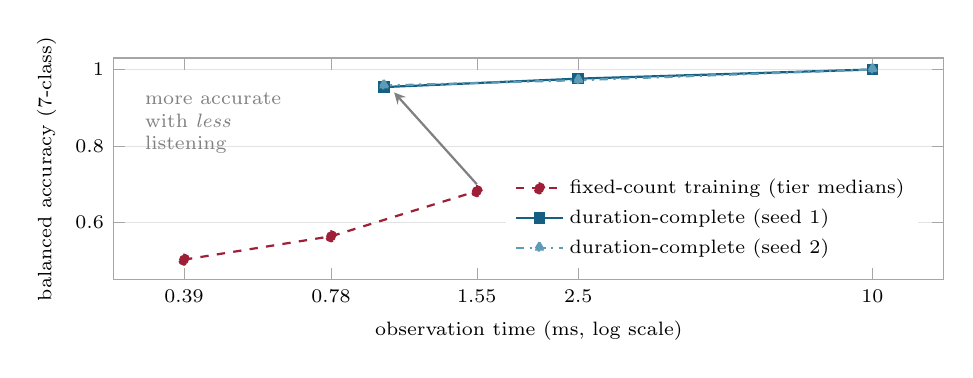
\begin{tikzpicture}
\begin{semilogxaxis}[width=\columnwidth,height=4.4cm,
  xmin=0.28,xmax=14,ymin=0.45,ymax=1.03,
  xlabel={\scriptsize observation time (ms, log scale)},
  ylabel={\scriptsize balanced accuracy (7-class)},
  xlabel style={font=\scriptsize}, ylabel style={font=\scriptsize},
  tick label style={font=\scriptsize},
  xtick={0.39,0.78,1.55,2.5,10}, xticklabels={0.39,0.78,1.55,2.5,10},
  legend style={font=\scriptsize,at={(0.97,0.05)},anchor=south east,draw=none},
  legend cell align=left]
\addplot[thick,oldc,mark=*,mark size=1.8pt,dashed] coordinates
  {(0.39,0.503) (0.78,0.564) (1.55,0.682)};
\addlegendentry{fixed-count training (tier medians)}
\addplot[thick,newc,mark=square*,mark size=1.7pt] coordinates
  {(1,0.954) (2.5,0.976) (10,1.000)};
\addlegendentry{duration-complete (seed 1)}
\addplot[thick,new2c,mark=triangle*,mark size=2pt,dashdotted] coordinates
  {(1,0.958) (2.5,0.972) (10,1.000)};
\addlegendentry{duration-complete (seed 2)}
\draw[-stealth,gray,thick] (axis cs:1.55,0.700) -- (axis cs:1.05,0.940);
\node[font=\scriptsize,gray,align=left,anchor=west] at (axis cs:0.31,0.86)
  {more accurate\\with \emph{less}\\listening};
\end{semilogxaxis}
\end{tikzpicture}
\caption{\textbf{Accuracy vs.\ observation time.} The identical
1.0M-parameter encoder trained on fixed-count data (tiers at their median
physical durations) and on duration-complete data (two seeds): more
accurate at every operating point with \emph{less} listening; at 10\,ms
every class reaches recall 1.000 on both seeds.}
\label{fig:attr}
\end{figure}

\begin{table}[t]\centering\scriptsize\setlength{\tabcolsep}{3pt}
\caption{Controls on the fixed-count corpus: no model-side intervention
approaches the effect of duration-complete data.}
\label{tab:controls}
\begin{tabular}{@{}llr@{}}
\toprule
Intervention (control corpus) & Metric & Effect \\
\midrule
Feature-eng.\ baseline, 50-trial search & worst-win.\ bal. & 0.743 \\
\quad its GSM recall, shortest tier & GSM recall & 0.49 \\
Our encoder, raw / normalized input & GSM recall & 0.34 / 0.45 \\
$3\times$ training budget & worst-win.\ bal. & 0.681 $\to$ 0.657 \\
Worst-case loss, wt.\ .05/.15/.40 & $\Delta$ w.-win. & $+.003$/$+.009$/$-.008$ \\
Worst-case loss, $3\times$ budget & $\Delta$ w.-win. & $+.055$ \\
\midrule
Duration-complete data, fixed encoder & shortest-tier bal. & 0.503 $\to$ 0.954 \\
\bottomrule
\end{tabular}
\end{table}

\section{Limitations}\label{sec:lim}
All data are synthetic; over-the-air validation remains future work
\cite{oshea2018}. The hop composition reproduces occupancy and timing
statistics, not the specification's selection kernel, and repeats verified
payload bits. Captures contain a single emitter; co-channel interference
and Doppler are absent. Confidence calibration \cite{guo2017} on held-out
data is required before escalation thresholds are meaningful, and the
full-system numbers above are an early snapshot at one third of the
training schedule.

\section{Conclusion}
The scanner's bargain---glance and be fooled, stare and go blind---was
never going to be resolved by a better glance. It is resolved by an architecture that can spend observation time
deliberately---classifying, modeling the clean channel, and judging its
own reliability at every dwell---and by training data whose windows
contain the rhythms that make that judgment learnable. With the model
frozen, duration-complete data moved the problem from 0.503 to 0.954 at
1\,ms; with the data frozen, no model-side intervention came close. When a
worst-case metric plateaus across model families, audit what the
observation window physically contains---and what the metric can
statistically display---before spending another epoch on the model.
Sometimes the signal is the noise---and sometimes the answer is to keep
listening.

\begin{thebibliography}{14}\footnotesize
\setlength{\itemsep}{0pt}
\bibitem{oshea2016} T.~J. O'Shea, J.~Corgan, and T.~C. Clancy,
``Convolutional radio modulation recognition networks,'' in \emph{Proc.
EANN}, 2016.
\bibitem{oshea2018} T.~J. O'Shea, T.~Roy, and T.~C. Clancy, ``Over-the-air
deep learning based radio signal classification,'' \emph{IEEE J. Sel.
Topics Signal Process.}, vol.~12, no.~1, 2018.
\bibitem{snell2017} J.~Snell, K.~Swersky, and R.~Zemel, ``Prototypical
networks for few-shot learning,'' in \emph{NeurIPS}, 2017.
\bibitem{he2022} K.~He, X.~Chen, S.~Xie, Y.~Li, P.~Doll\'ar, and
R.~Girshick, ``Masked autoencoders are scalable vision learners,'' in
\emph{CVPR}, 2022.
\bibitem{vincent2010} P.~Vincent, H.~Larochelle, I.~Lajoie, Y.~Bengio, and
P.-A. Manzagol, ``Stacked denoising autoencoders: Learning useful
representations in a deep network with a local denoising criterion,''
\emph{J. Mach. Learn. Res.}, vol.~11, 2010.
\bibitem{devries2018} T.~DeVries and G.~W. Taylor, ``Learning confidence
for out-of-distribution detection in neural networks,''
arXiv:1802.04865, 2018.
\bibitem{hendrycks2017} D.~Hendrycks and K.~Gimpel, ``A baseline for
detecting misclassified and out-of-distribution examples in neural
networks,'' in \emph{ICLR}, 2017.
\bibitem{geifman2017} Y.~Geifman and R.~El-Yaniv, ``Selective
classification for deep neural networks,'' in \emph{NeurIPS}, 2017.
\bibitem{guo2017} C.~Guo, G.~Pleiss, Y.~Sun, and K.~Q. Weinberger, ``On
calibration of modern neural networks,'' in \emph{ICML}, 2017.
\bibitem{teerapittayanon2016} S.~Teerapittayanon, B.~McDanel, and H.~T.
Kung, ``BranchyNet: Fast inference via early exiting from deep neural
networks,'' in \emph{ICPR}, 2016.
\bibitem{huang2018} G.~Huang, D.~Chen, T.~Li, F.~Wu, L.~van~der~Maaten,
and K.~Q. Weinberger, ``Multi-scale dense networks for resource efficient
image classification,'' in \emph{ICLR}, 2018.
\bibitem{loshchilov2019} I.~Loshchilov and F.~Hutter, ``Decoupled weight
decay regularization,'' in \emph{ICLR}, 2019.
\bibitem{btcore} Bluetooth SIG, \emph{Bluetooth Core Specification},
Version 6.3, 2026.
\bibitem{ts45002} 3GPP, ``Multiplexing and multiple access on the radio
path,'' TS 45.002, Rel.~19, 2026.
\end{thebibliography}

\end{document}
